\PassOptionsToPackage{table}{xcolor}
\documentclass[12pt,letterpaper,twocolumn,openany,nodeprecatedcode,bg=none]{dndbook}
\usepackage[english]{babel}
\usepackage[utf8]{inputenc}
\usepackage{longtable,booktabs,array}
\usepackage{calc}
\usepackage{etoolbox}
\usepackage{caption}
\usepackage{float}
\usepackage{graphicx}
\usepackage{needspace}
\usepackage{tikz}

% Reset zebra striping at the start of every table
\AtBeginEnvironment{longtable}{\rowcolors{1}{white}{gray!10}\small}
\AtBeginEnvironment{table}{\rowcolors{1}{white}{gray!10}}

\providecommand{\pandocbounded}[1]{#1}
\providecommand{\tightlist}{%
  \setlength{\itemsep}{0pt}\setlength{\parskip}{0pt}}

\captionsetup{labelformat=empty}
\setcounter{secnumdepth}{0}
\setlength{\parindent}{0pt}
\setlength{\parskip}{0.5\baselineskip}
\setlength{\headheight}{15pt}

% Prevent orphaned subsections
\let\oldsubsection\subsection
\renewcommand{\subsection}[1]{%
  \needspace{5\baselineskip}%
  \oldsubsection{#1}%
}

\begin{document}
\onecolumn

      \title{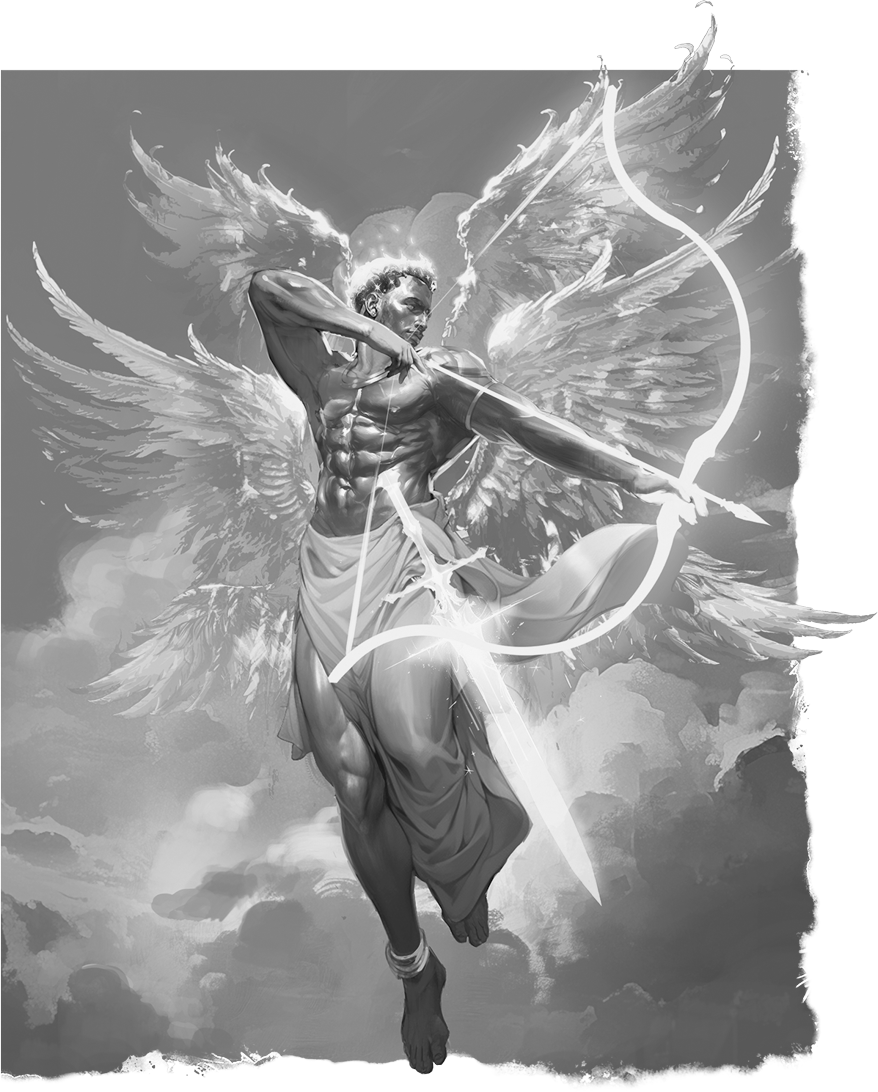
\includegraphics[width=0.9\textwidth,height=0.55\textheight,keepaspectratio]{solar5e-bw.png}\\[1.5cm]Mystic
of the Sun}
  \author{Class Handbook}
\date{}
\maketitle


\clearpage
\thispagestyle{empty}
\begin{center}
\vspace*{\fill}
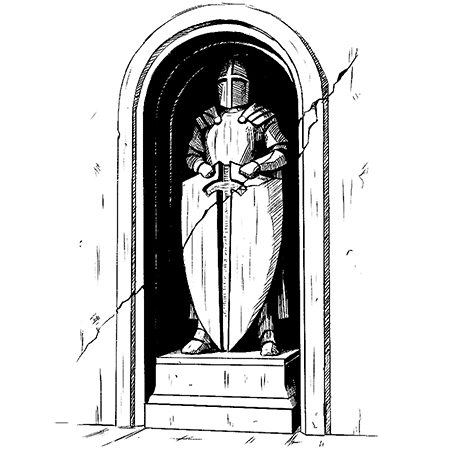
\includegraphics[width=\textwidth,height=0.85\textheight,keepaspectratio]{holyPaladin.jpg}\par
\vspace{0.4cm}
{\itshape By the holy light!}\par
\vspace*{\fill}
\end{center}

\clearpage
\twocolumn

\section{Mystic (Sun)}\label{mystic-sun}

\subsection{Core Mystic (Sun) Traits}\label{core-mystic-sun-traits}

\needspace{11\baselineskip}

{\def\LTcaptype{none} % do not increment counter
\begin{table}[!htbp]
\centering
\begin{tabular}{@{}
  >{\raggedright\arraybackslash}p{(\linewidth - 2\tabcolsep) * \real{0.3662}}
  >{\raggedright\arraybackslash}p{(\linewidth - 2\tabcolsep) * \real{0.6338}}@{}}
\toprule\noalign{}
\begin{minipage}[b]{\linewidth}\raggedright
\textbf{Primary Ability}
\end{minipage} & \begin{minipage}[b]{\linewidth}\raggedright
Charisma
\end{minipage} \\
\midrule\noalign{}
\textbf{Hit Points} & 1d6 \\
\textbf{Saving Throw Proficiencies} & Wisdom, Charisma \\
\textbf{Skill Proficiencies} & Choose 2 skills \\
\textbf{Weapon Proficiencies} & Choose 2 categories \\
\textbf{Starting Equipment} & Padded Jacket, Longbow, Dagger, Golden
Amulet \\
\bottomrule\noalign{}
\end{tabular}
\end{table}
}

\subsection{Mystic (Sun) Features}\label{mystic-sun-features}

\needspace{20\baselineskip}

{\def\LTcaptype{none} % do not increment counter
\begin{table}[!htbp]
\centering
\begin{tabular}{@{}
  >{\raggedright\arraybackslash}p{(\linewidth - 4\tabcolsep) * \real{0.1190}}
  >{\raggedright\arraybackslash}p{(\linewidth - 4\tabcolsep) * \real{0.2619}}
  >{\raggedright\arraybackslash}p{(\linewidth - 4\tabcolsep) * \real{0.6190}}@{}}
\toprule\noalign{}
\begin{minipage}[b]{\linewidth}\raggedright
Level
\end{minipage} & \begin{minipage}[b]{\linewidth}\raggedright
Proficiency
\end{minipage} & \begin{minipage}[b]{\linewidth}\raggedright
Class Features
\end{minipage} \\
\midrule\noalign{}
1 & +2 & Spellcasting, Radiant Aura \\
2 & +2 & --- \\
3 & +2 & Ability Bonus \\
4 & +2 & --- \\
5 & +2 & --- \\
6 & +2 & --- \\
7 & +2 & Ability Bonus \\
8 & +2 & --- \\
9 & +3 & --- \\
10 & +3 & --- \\
\bottomrule\noalign{}
\end{tabular}
\end{table}
}

\subsection{Level 1: Spellcasting}\label{level-1-spellcasting}

You can cast spells from the Mystic (Sun) spell list. Wisdom or Charisma
is your casting ability, chosen when you cast a spell. You know two
cantrips.

You prepare a number of spells equal to your total number of spell
slots. You may change your prepared spells after an extended period of
downtime.

You regain all expended spell slots when you finish a long rest. Once
per day, you may regain 1 expended spell slot when you finish a short
rest.

\subsection{Spell Slots by Level}\label{spell-slots-by-level}

\needspace{20\baselineskip}

{\def\LTcaptype{none} % do not increment counter
\begin{table}[!htbp]
\centering
\begin{tabular}{@{}
  >{\raggedright\arraybackslash}p{(\linewidth - 6\tabcolsep) * \real{0.3571}}
  >{\raggedright\arraybackslash}p{(\linewidth - 6\tabcolsep) * \real{0.2143}}
  >{\raggedright\arraybackslash}p{(\linewidth - 6\tabcolsep) * \real{0.2143}}
  >{\raggedright\arraybackslash}p{(\linewidth - 6\tabcolsep) * \real{0.2143}}@{}}
\toprule\noalign{}
\begin{minipage}[b]{\linewidth}\raggedright
Level
\end{minipage} & \begin{minipage}[b]{\linewidth}\raggedright
1
\end{minipage} & \begin{minipage}[b]{\linewidth}\raggedright
2
\end{minipage} & \begin{minipage}[b]{\linewidth}\raggedright
3
\end{minipage} \\
\midrule\noalign{}
1 & 2 & -- & -- \\
2 & 2 & -- & -- \\
3 & 3 & -- & -- \\
4 & 3 & -- & -- \\
5 & 4 & 2 & -- \\
6 & 4 & 2 & -- \\
7 & 4 & 3 & -- \\
8 & 4 & 3 & -- \\
9 & 4 & 3 & 2 \\
10 & 4 & 3 & 2 \\
\bottomrule\noalign{}
\end{tabular}
\end{table}
}

\subsection{Level 1: Radiant Aura}\label{level-1-radiant-aura}

You gain the Light cantrip.

When you cast the cantrip, it sheds bright sunlight rather than dim
light. On your turn, you add your Charisma bonus to weapon damage rolls
against targets in the spell's area. If the target is undead, that bonus
increases to your Charisma modifier + your level.

\subsection{Level 3: Ability Bonus}\label{level-3-ability-bonus}

You gain a +1 bonus to two different abilities of your choice.

\subsection{Level 7: Ability Bonus}\label{level-7-ability-bonus}

You gain a +1 bonus to two different abilities of your choice.

\clearpage

\section{Mystic (Sun) Spells}\label{mystic-sun-spells}

The tables are numbered for random spell selection.

\subsection{Cantrips}\label{cantrips}

\needspace{13\baselineskip}

{\def\LTcaptype{none} % do not increment counter
\begin{table}[!htbp]
\centering
\begin{tabular}{@{}
  >{\raggedright\arraybackslash}p{(\linewidth - 2\tabcolsep) * \real{0.1667}}
  >{\raggedright\arraybackslash}p{(\linewidth - 2\tabcolsep) * \real{0.8333}}@{}}
\toprule\noalign{}
\begin{minipage}[b]{\linewidth}\raggedright
d6
\end{minipage} & \begin{minipage}[b]{\linewidth}\raggedright
Cantrip
\end{minipage} \\
\midrule\noalign{}
1 & Chromatic Flare \\
2 & Light* \\
3 & Sacred Flame \\
4 & Spare the Dying \\
5 & Thaumaturgy \\
6 & True Strike \\
\bottomrule\noalign{}
\end{tabular}
\end{table}
}

\subsection{Level 1 Spells}\label{level-1-spells}

\needspace{9\baselineskip}

{\def\LTcaptype{none} % do not increment counter
\begin{table}[!htbp]
\centering
\begin{tabular}{@{}
  >{\raggedright\arraybackslash}p{(\linewidth - 2\tabcolsep) * \real{0.2000}}
  >{\raggedright\arraybackslash}p{(\linewidth - 2\tabcolsep) * \real{0.8000}}@{}}
\toprule\noalign{}
\begin{minipage}[b]{\linewidth}\raggedright
d4
\end{minipage} & \begin{minipage}[b]{\linewidth}\raggedright
Level 1
\end{minipage} \\
\midrule\noalign{}
1 & Bless \\
2 & Color Spray \\
3 & Cure Wounds \\
4 & Guiding Bolt \\
\bottomrule\noalign{}
\end{tabular}
\end{table}
}

\subsection{Level 2 Spells}\label{level-2-spells}

\needspace{9\baselineskip}

{\def\LTcaptype{none} % do not increment counter
\begin{table}[!htbp]
\centering
\begin{tabular}{@{}
  >{\raggedright\arraybackslash}p{(\linewidth - 2\tabcolsep) * \real{0.1500}}
  >{\raggedright\arraybackslash}p{(\linewidth - 2\tabcolsep) * \real{0.8500}}@{}}
\toprule\noalign{}
\begin{minipage}[b]{\linewidth}\raggedright
d4
\end{minipage} & \begin{minipage}[b]{\linewidth}\raggedright
Level 2
\end{minipage} \\
\midrule\noalign{}
1 & Augury \\
2 & Hold Creature \\
3 & Restorative Touch \\
4 & Scorching Ray \\
\bottomrule\noalign{}
\end{tabular}
\end{table}
}

\subsection{Level 3 Spells}\label{level-3-spells}

\needspace{9\baselineskip}

{\def\LTcaptype{none} % do not increment counter
\begin{table}[!htbp]
\centering
\begin{tabular}{@{}
  >{\raggedright\arraybackslash}p{(\linewidth - 2\tabcolsep) * \real{0.1579}}
  >{\raggedright\arraybackslash}p{(\linewidth - 2\tabcolsep) * \real{0.8421}}@{}}
\toprule\noalign{}
\begin{minipage}[b]{\linewidth}\raggedright
d4
\end{minipage} & \begin{minipage}[b]{\linewidth}\raggedright
Level 3
\end{minipage} \\
\midrule\noalign{}
1 & Dispel Magic \\
2 & Revivify \\
3 & Speak with Dead \\
4 & Spirit Guardians \\
\bottomrule\noalign{}
\end{tabular}
\end{table}
}

\section{Mystic (Sun) Spell List}\label{mystic-sun-spell-list}

Spells descriptions are listed below.

\subsection{Augury}\label{augury}

\textbf{Level:} 2

You receive an omen from mystical forces about the results of a course
of action that you plan to take within the next 30 minutes. The DM
chooses whether to answer weal, woe, or a mix of the two, depending on
the most likely outcome of the action.

\subsection{Bless}\label{bless}

\textbf{Level:} 1

\textbf{Range:} 30 feet

\textbf{Duration:} Concentration, up to 1 minute

You bless up to three creatures within range. A blessed creature adds
1d4 to their attack rolls and saves.

\subsection{Chromatic Flare}\label{chromatic-flare}

\textbf{Level:} Cantrip

\textbf{Range:} 120 feet

You send a bolt of scintillating, chromatic energy at a foe. Make a
ranged attack against the target. On a hit, the target takes 1d8 radiant
damage and you are invisible to it for 1d3 rounds.

The damage increases to 2d8 radiant damage at level 5 and 3d8 radiant
damage at level 9.

\subsection{Color Spray}\label{color-spray}

\textbf{Level:} 1

\textbf{Range:} Self

Waves of chromatic energy erupt from your outstretched hands, dazzling
creatures before you. Each creature in a 15-foot cone projected from you
makes a Wisdom saving throw, taking 2d6 radiant damage on a failed save
or half damage on a successful one.

If a creature fails the save, it is blinded for 1 round.

\subsection{Cure Wounds}\label{cure-wounds}

\textbf{Level:} 1

\textbf{Range:} Touch

A creature you touch regains 2d8 + your spellcasting bonus hit points.

The healing increases to 4d8 + your spellcasting bonus if you use a
level 2 slot and 6d8 + your spellcasting bonus if you use a level 3
slot.

\subsection{Dispel Magic}\label{dispel-magic}

\textbf{Level:} 3

\textbf{Range:} 120 feet

Choose one creature, object, or magical effect within range. Any ongoing
spell of level 3 or lower on the target ends. For each ongoing spell of
level 4 or higher on the target, make an ability check using your
spellcasting ability (DC 10 plus that spell's level). On a successful
check, the spell ends.

\newpage

\subsection{Guiding Bolt}\label{guiding-bolt}

\textbf{Level:} 1

\textbf{Range:} 120 feet

\textbf{Duration:} 1 round

You hurl a bolt of light toward a creature within range. Make a ranged
spell attack against the target. On a hit, it takes 4d6 radiant damage
and the next attack against the target gains advantage.

The damage increases to 6d6 radiant damage if you use a level 2 slot and
8d6 radiant damage if you use a level 3 slot.

\subsection{Hold Creature}\label{hold-creature}

\textbf{Level:} 2

\textbf{Range:} 60 feet

\textbf{Duration:} Concentration, up to 1 minute

Choose a creature that you can see within range. The target must succeed
on a Wisdom saving throw or become paralyzed. At the end of each of its
turns, the target repeats the save, ending the spell on itself on a
success.

If you use a level 3 slot to cast this spell, you can target two
creatures.

\subsection{Light}\label{light}

\textbf{Level:} Cantrip

\textbf{Range:} Touch

\textbf{Duration:} 1 hour

An object you touch sheds dim light in a 30-foot radius and Dim Light
for an additional 20 feet. The spell ends if you cast it again.

\subsection{Restorative Touch}\label{restorative-touch}

\textbf{Level:} 2

\textbf{Range:} Touch

You touch a creature and end one condition on it: blinded, paralyzed, or
poisoned.

\subsection{Revivify}\label{revivify}

\textbf{Level:} 3

\textbf{Range:} Touch

You touch a creature. If that creature died within the last minute, it
returns to life, restores one failed death save, and regains 1 hit
point. It cannot restore failed death saves again until it finishes a
long rest.

\subsection{Sacred Flame}\label{sacred-flame}

\textbf{Level:} Cantrip

\textbf{Range:} 60 feet

Flame-like radiance descends on a creature that you can see within
range. The target must succeed on a Dexterity saving throw or take 1d8
radiant damage.

The damage increases to 2d8 radiant damage at level 5 and 3d8 radiant
damage at level 9.

\subsection{Scorching Ray}\label{scorching-ray}

\textbf{Level:} 2

\textbf{Range:} 120 feet

You hurl three fiery rays. You can hurl them at one target within range
or at several. Make a ranged spell attack for each ray. On a hit, the
target takes 2d6 fire or radiant damage, your choice.

If you cast this spell with a level 3 slot, the damage increases to 3d6.

\subsection{Spare the Dying}\label{spare-the-dying}

\textbf{Level:} Cantrip

\textbf{Range:} 30 feet

Choose a living creature within range that has 0 hit points. It regains
1 hit point.

\subsection{Speak with Dead}\label{speak-with-dead}

\textbf{Level:} 3

\textbf{Range:} 10 feet

\textbf{Duration:} 10 minutes

You touch a corpse and attempt to commune with its spirit. If its spirit
can be contacted, you contact it through mystical means.

Until the spell ends, you can ask the spirit of the corpse up to five
questions. The spirit knows only what it knew in life, including the
languages it knew. The spirit is under no compulsion to offer a truthful
answer if you are antagonistic toward it or it recognizes you as an
enemy.

The dead often demand a service in return for the information they
provide. If you accept such a deal, you cannot cast this spell again
until you complete the task or make a good faith effort to do so.

\newpage

\subsection{Spirit Guardians}\label{spirit-guardians}

\textbf{Level:} 3

\textbf{Duration:} Concentration, up to 10 minutes

Protective spirits flit around you in a 15-foot radius. This radius
moves with you.

When you cast this spell, you can designate creatures to be unaffected
by it. The designated creatures ignore the spell's effects.

A creature's speed is halved while within the spell's area. A creature
that starts its turn in the area takes 2d8 radiant damage. A creature
can take this damage only once per round.

\subsection{Thaumaturgy}\label{thaumaturgy}

\textbf{Level:} Cantrip

\textbf{Range:} 30 feet

\textbf{Duration:} Up to 1 minute

You manifest a minor wonder within range. You can create minor
illusions, alter one of your physical traits, change the sound or volume
of your voice, and otherwise make cosmetic changes to yourself or an
object in range. The spell ends if you cast it again.

\subsection{True Strike}\label{true-strike}

\textbf{Level:} Cantrip

\textbf{Range:} Self

Guided by a flash of magical insight, you make one attack with a weapon.

The attack uses your spellcasting ability for the attack and damage
rolls instead of using Strength or Dexterity.

You deal an additional 1d6 radiant damage with this attack at level 5
and 2d6 radiant damage at level 9.

\onecolumn

\clearpage
\thispagestyle{empty}
\begin{center}
\vspace*{\fill}
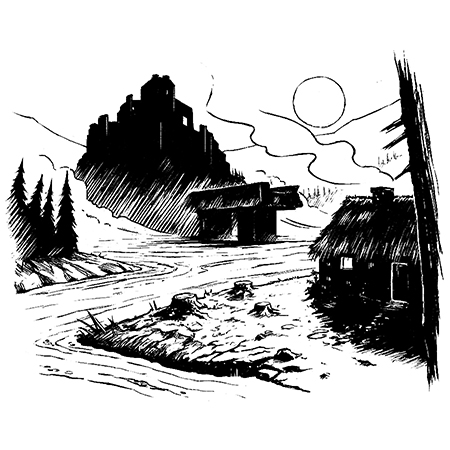
\includegraphics[width=0.7\textwidth,keepaspectratio]{risingSun.jpg}\par
\vspace{0.4cm}
{\itshape The sun is warmth and the giver of life itself.}\par
\vspace*{\fill}
\end{center}

\end{document}